\begin{frame}[fragile]{Redirections}

\begin{columns}

\column{0.38\linewidth}
\begin{figure}
    \centering
    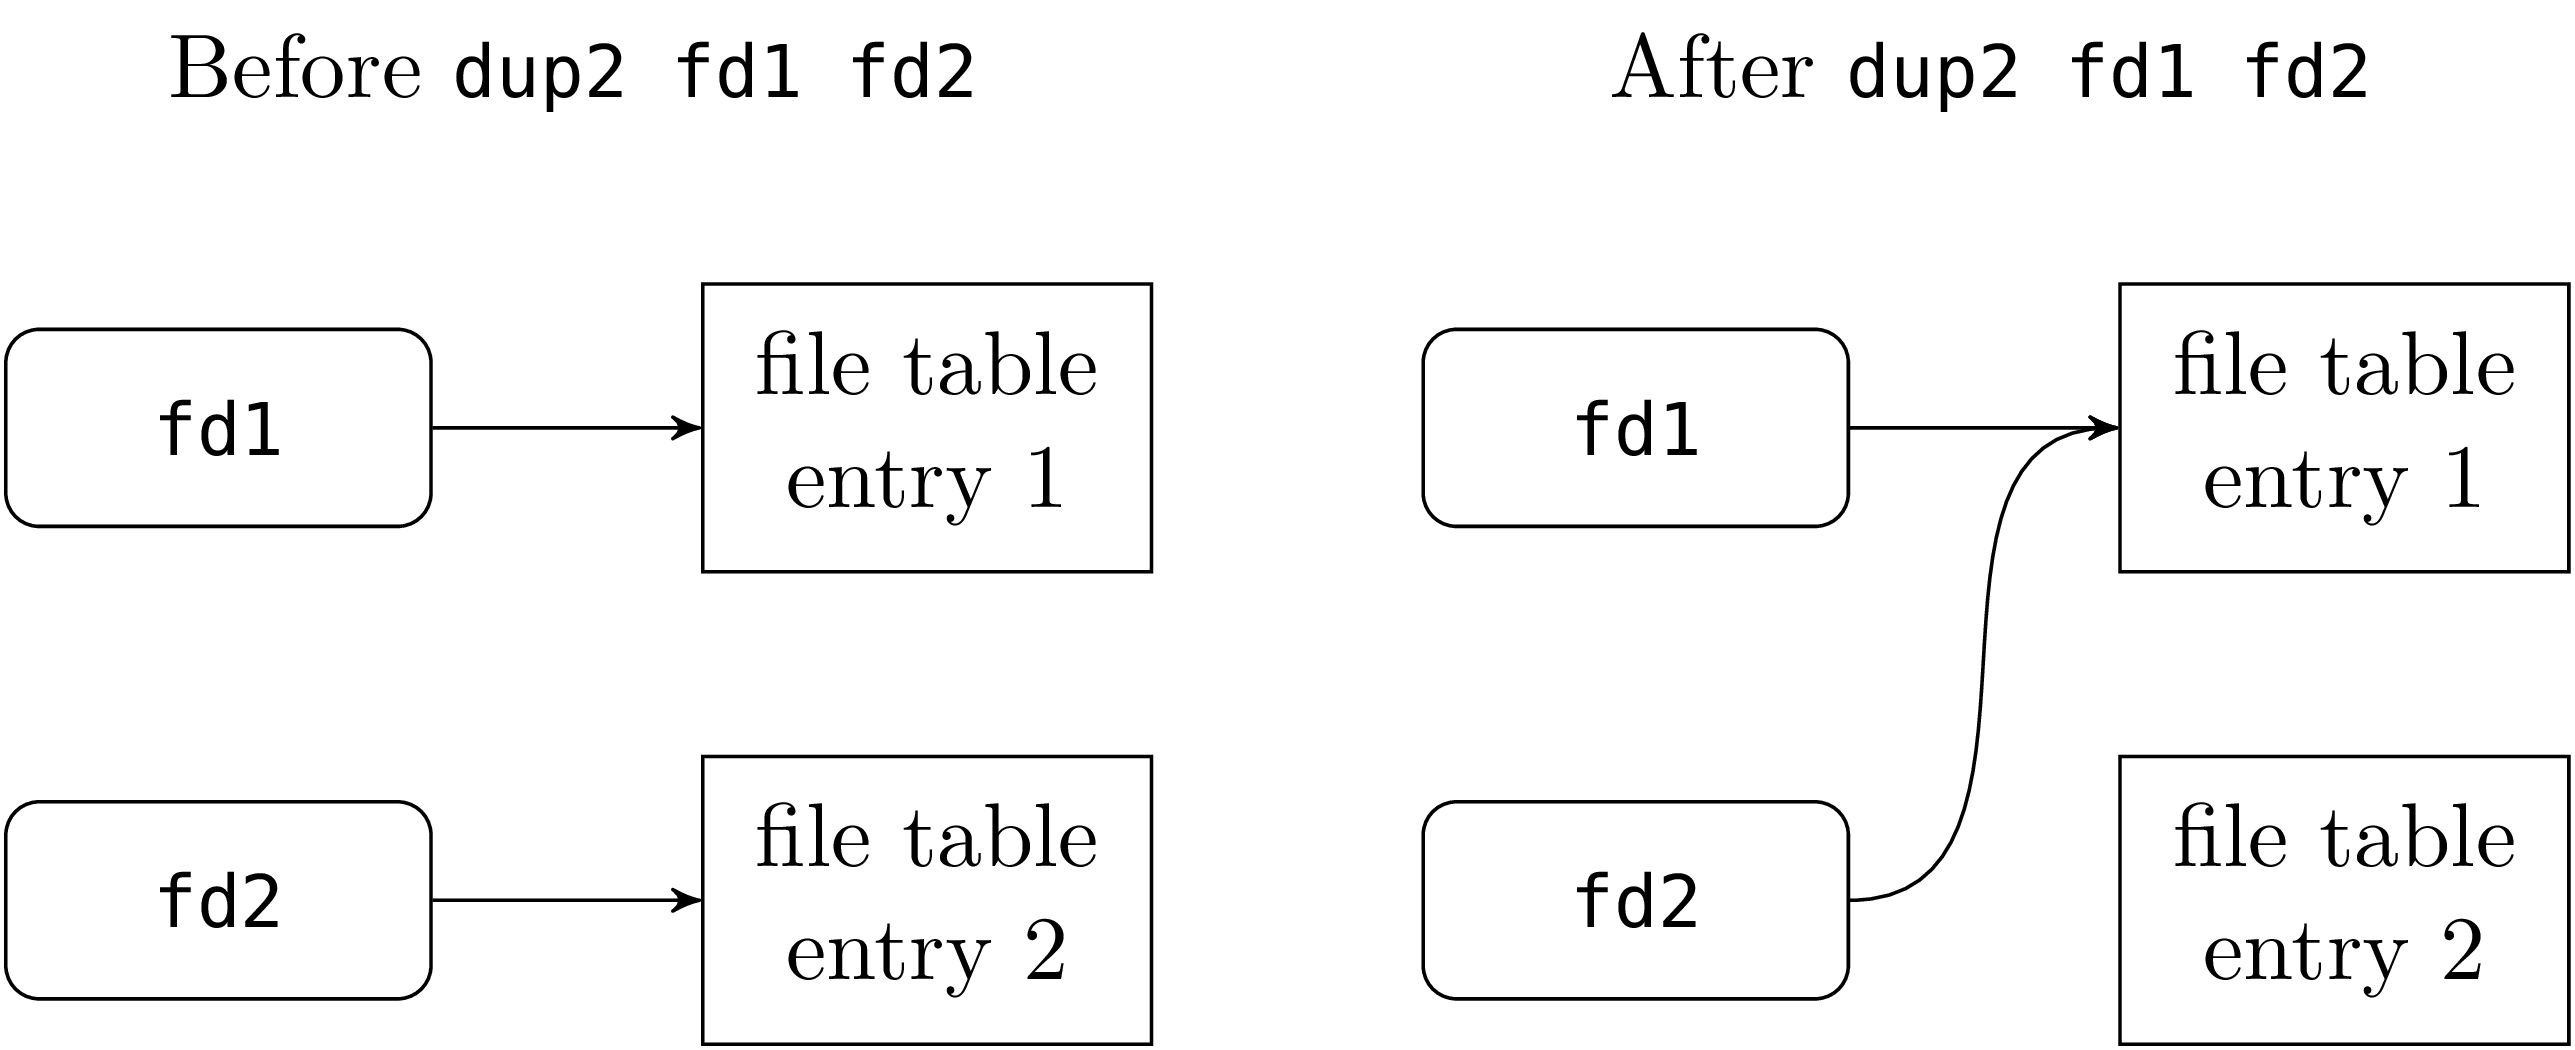
\includegraphics[width=\textwidth]{slides/images/dup2.png}
\end{figure}

\column{0.58\linewidth}
\\
\subtt{Fonction Unix:}
\begin{lstlisting}
val dup2 : file_descr -> file_descr -> unit
\end{lstlisting}

\end{columns}

\subtt{Implémentation :}

\begin{lstlisting}
let redirection_entree target =
  let fd = Unix.openfile target [ Unix.O_RDONLY ] 0 in
  Unix.dup2 fd Unix.stdin;
  Unix.close fd

let redirection_sortie target =
  let fd = Unix.openfile target [ Unix.O_CREAT ; 
                                  Unix.O_TRUNC ; 
                                  Unix.O_WRONLY ] 0o660
  in
  Unix.dup2 fd Unix.stdout;
  Unix.close fd
\end{lstlisting}

\end{frame}

\begin{frame}[fragile]{Tubes}

\subtt{Fonction Unix :}
\begin{lstlisting}
val pipe : unit -> file_descr * file_descr
\end{lstlisting}

\subtt{Implémentation :}
\begin{lstlisting}
let pipe_cmd (a: Command.t) (b: Command.t) =
  let fd_in, fd_out = Unix.pipe () in
  match Unix.fork () with
  | 0 ->
      Unix.dup2 fd_out Unix.stdout;
      Unix.close fd_out;
      Unix.close fd_in;
      interprete a
  | _ ->
      Unix.dup2 fd_in Unix.stdin;
      Unix.close fd_out;
      Unix.close fd_in;
      interprete b
\end{lstlisting}

\end{frame}